\par The next consideration to be made was supplying power. In the pursuit of making out devices truly wireless, we were determined to have all the end-point devices be completely battery operated. Though the XBee RF modules themselves use minimal power even while transmitting, an efficient power supply would be necessary for prolonged operation. 
	\begin{wrapfigure}[]{l}{2.5in}
		\includegraphics[width=2in]{lm317.jpg}
		\caption{\small LM317 Linear Regulator (TH)}
	\end{wrapfigure}
	\paragraph{\normalsize LM317 Linear Voltage Regulator \hspace{1.5em}} 
	The LM317 is an IC designed to maintain a constant voltage level. Voltage regulators usually have an input voltage range, but for the LM317 voltage regulator, the range is not specified because it has no ground connection. It has an output voltage range from 1.2 V to 37 V at 1.5 A. Since it is a linear regulator, the output voltage is always lower than input. The LM317 is used in our project to power the XBee modules which require a supply voltage between 2.1 V and 3.6 V. We designed a circuit incorporating the LM317 to output 3.3 V, which is ideal to power our devices. \\ 
	\begin{figure}[h]
		\centering
		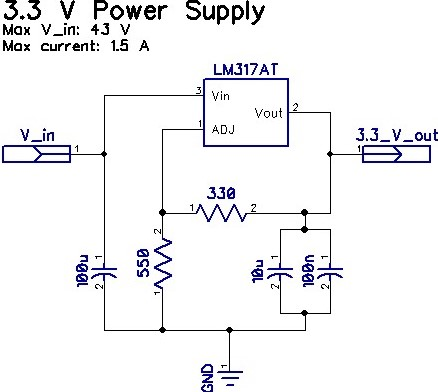
\includegraphics[width=3in]{33vsource.jpg}
		\caption{Complete power supply circuit.}
		\label{3v_circuit}
	\end{figure}
	\par As in figure \ref{3v_circuit}, the values we know are V\textsubscript{o} = 1.2 V, V\textsubscript{out} = 3.3 V and setting R1 = 330 $\Omega$.  The value of Iadj is very small hence it can have considered negligible. The value of R2 came to 550 $\Omega$. We then added the C1 = 100 $\mu$F, C2 = 0.1 $\mu$F and C3 = 10 $\mu$F for the improvement of transient response of a system to change from steady state. 
	
	\paragraph{\normalsize LM7805 5V Voltage Regulator}
	To power our devices that require a 5 volt source such as the MQ-6 LP gas sensor, we chose to design a circuit around the LM7805 voltage regulator. This regulator has an input range of 5 to 18 volts, ideal for out 6 volt battery packs, and produces a constant 5 volt output. 

